\documentclass[12pt]{aiaa-tc}
\usepackage{tex4ht}
\usepackage[english]{babel}
\usepackage{epstopdf}
\usepackage{epsfig}
\usepackage{graphicx}
\usepackage{fancyhdr}
\usepackage{color}
\usepackage{caption}
\usepackage{amsmath}
\usepackage{amssymb}
\usepackage{tabularx}
\usepackage{subfigure}
\usepackage{enumerate}
\usepackage{booktabs}
\usepackage{colortbl}
\usepackage{tabbing}
\usepackage{fltpage}
\usepackage[colorlinks]{hyperref}


\setlength{\parindent}{0in}
\addtolength{\parskip}{\baselineskip}
\renewcommand{\baselinestretch}{1}
\newcommand{\dg}{^\circ}

\begin{document}

\title{Aircraft B: inertial coupling nonlinearity in flight dynamics}
\maketitle

The nonlinear flight dynamics equations of motion encompass a variety of sources of
nonlinearity: aerodynamic, inertial and kinematic.  The aerodynamic components of these
equations usually consist of tabular datasets, capturing the nonlinear variations in
aerodynamic load with angle of attack and other state and control variables.  Much of the
nonlinear flight dynamics of manoeuvring aircraft arises from these aerodynamic
nonlinearities, which typically come into play at higher angles of attack.

The `aircraft B� example illustrates the use of bifurcation analysis to identify flight
dynamics nonlinearity arising from {\em inertial coupling}, rather than aerodynamic
nonlinearity.  The model uses a constant-coefficient aerodynamic formulation that,
although incorporating a certain element of nonlinearity, avoids the full nonlinearity
inherent in tabular data.

Observation of the rotational equations of motion of an aircraft in flight reveals that the
inertial terms become significant as rotation rate increases.  Here, some background as to
the origin and nature of inertial coupling is given.

During conventional wings-level or turning flight, $\beta \!\approx\!
0$ ($v \!\approx\! 0$).  This results in aerodynamic flows that are
(at least in the absence of high angle of attack aerodynamic coupling)
symmetric with respect to the aircraft x-z plane.  However, when
rolling about the body x-axis at non-zero $\alpha$, the sideslip
velocity, $v$, becomes non-zero so that $\beta$ becomes non-zero.  As
the roll continues, it kinematically converts $\alpha$ into $\beta$: a
$90\dg$ body-axis roll leads to complete conversion of angle of attack
into sideslip.

As the magnitude of $\beta$ grows, so the forces and moments in the
lateral-directional sense (x-y and y-z planes) increase, thus
eliminating the earlier symmetry.  Apart from hampering the roll
motion intended by the pilot, and thus increasing pilot workload, this may induce
undesirable
bifurcationary phenomena such as lateral-directional departure.  The
higher the value of $\alpha$ at the start of the roll, the more severe
the magnitude and consequences of this kinematic coupling.

In order to eliminate kinematic coupling and its consequences, pilots
may roll the aircraft about the velocity vector --- particularly
when operating at moderate to high $\alpha$.  This is achieved by a
combination of body-axis roll rate, $p$, and body-axis yaw rate, $r$,
to give a velocity vector (or wind axis) roll rate of $p_{w}$.  Figure
\ref{fig:velroll} shows that $p_{w}$ can be written:

\begin{equation}
p_{w} = \frac{p}{\cos\alpha} \label{eq:p_w_vvr}
\end{equation} and that
\begin{equation}
r = p \tan\alpha. \label{eq:r_vvr}
\end{equation}

\vspace{1cm}

\begin{figure}[ht]
\centering
  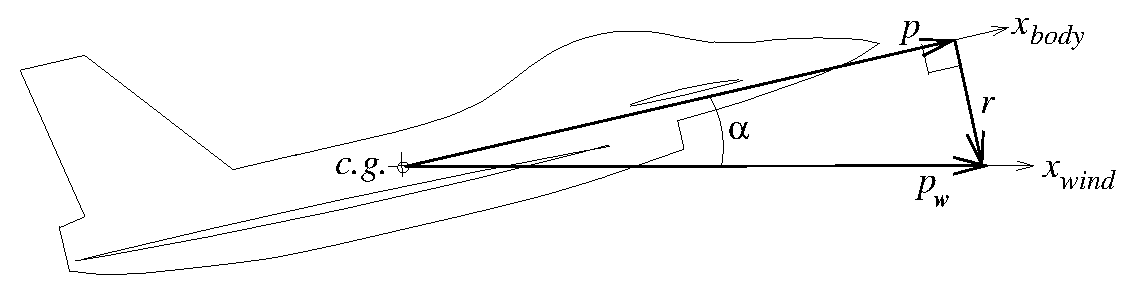
\includegraphics[height=3cm]{velroll.eps}\\
  \caption{Velocity vector roll components.}\label{fig:velroll}
\end{figure}

\vspace{1cm}

Such a manoeuvre maintains a constant $\alpha$ and $\beta$ but
unfortunately it may induce `inertial coupling': the tendency to align
the rotating air vehicle perpendicular to the axis of rotation, thus
creating large pitching moments.  To appreciate the cause of this
phenomenon, consider the inertial coupling term within equation
(\ref{eq:qdot}), $\frac{I_{zz}-I_{xx}}{I_{yy}}rp$.  Multiplying by
$I_{yy}$ gives the term the dimension of a moment; denoting this
pitching moment contribution due to inertial coupling as $M_{IC}$, we have:

\begin{equation}
M_{IC}=\left( I_{zz}-I_{xx} \right) rp \label{eq:IC1}
\end{equation}

Substituting equations (\ref{eq:p_w_vvr}) and (\ref{eq:r_vvr}) into
equation (\ref{eq:IC1}) allows the latter to be written as:

\begin{equation}
M_{IC} = \left( I_{zz}-I_{xx} \right) p_{w}^{2}
\end{equation}
\begin{equation}
\frac{\sin2\alpha}{2} \label{eq:IC2}
\end{equation}

For fighter aircraft configurations, $I_{zz} \!>\! I_{xx}$.  Thus it
may be observed from equation (\ref{eq:IC2}) that $M_{IC}$ is always
positive for positive angle of attack, and {\em vice versa}.  So if a
rapid roll is commanded at positive $\alpha$, a strong nose-up pitching
moment will develop.  This may lead to saturation of nose-down control
authority --- particularly in the stall/post-stall regimes and
especially so for aircraft with relaxed static stability --- and
possible loss of vehicle control \cite{Anderson:85,Alcorn_etal:96}.

Inertial coupling manifests itself not only during velocity vector
rolls at high $\alpha$.  Destabilising yawing moments can arise from
combined rolling and pitching.  From equation (\ref{eq:rdot}) it is
evident that the main inertial contribution to the yawing moment
(observing that the $qr$ term is small because $I_{xz}$ is usually
small) may be written:

\begin{equation}
N_{IC} = \left( I_{xx}-I_{yy} \right) pq  \label{eq:IC3}
\end{equation}

Consider a nose-up pitch rate (positive $q$), noting that for a
fighter aircraft $I_{yy} \!\gg\! I_{xx}$: equation (\ref{eq:IC3}) then
demonstrates that $N_{IC}$ will oppose the roll rate demanded in a
co-ordinated manoeuvre.  To avoid kinematic coupling, such a roll
should be about the velocity vector so that, from equation
(\ref{eq:r_vvr}), $r \!=\! p\tan\alpha$.  Under this condition, equation
(\ref{eq:IC3}) can then be arranged as:

\begin{equation}
N_{IC} = \frac{\left( I_{xx}-I_{yy} \right) rq}{\tan\alpha}\label{eq:IC4}
\end{equation}

For manoeuvres in which $0\dg \!<\! \alpha \!<\! 90\dg$ and pitch rate
is positive, the sign of $N_{IC}$ opposes that necessary for velocity
axis rolling (i.e.\ if a positive roll rate, $p$, is desired then $r
\!=\! p\tan\alpha$ requires a positive $r$; but as the rolling builds
up, so the inertial coupling inhibits this).  The result
\cite{Alcorn_etal:96} is the generation of sideslip that may
destabilise the aircraft (kinematic coupling) and lead to loss of
control at high angles of attack.

An interesting account of incidents due to inertial (and other)
coupling in various aircraft is given in \cite{Day:97}.

\bibliography{inertia}
\bibliographystyle{aiaa}

\end{document}
